\chapter{The Star Formation Rate at Galactic Scales: Observations}
\label{ch:sflaw_obs}

\marginnote{
\textbf{Suggested background reading:}
\begin{itemize}
\item \href{http://adsabs.harvard.edu/abs/2012ARA\%26A..50..531K}{Kennicutt, R.~C., \& Evans, N.~J. 2012, ARA\&A, 50, 531}, sections $5-6$ \nocite{kennicutt12a}
\end{itemize}
\textbf{Suggested literature:}
\begin{itemize}
\item \href{http://adsabs.harvard.edu/abs/2010AJ....140.1194B}{Bigiel et al., 2010, ApJ, 709, 191} \nocite{bigiel10a}
\item \href{http://adsabs.harvard.edu/abs/2013AJ....146...19L}{Leroy et al., 2013, ApJ, 146, 19} \nocite{leroy13a}
\end{itemize}
}

In the previous chapter we discussed observations of the bulk properties of giant molecular clouds. Now we will discuss the correlation of gas with star formation, a topic known loosely as star formation "laws". This chapter will focus on the observational situation, and the following one will focus on theoretical models that attempt to make sense of the observations. This is an extremely active area of research, and much of the available data is only a few years old. Most of the models are of similarly recent vintage. The central questions with which all of these models and data are concerned are: what determines the rate at which a galaxy transforms its gas content into stars? What determines where in the galaxy, both in terms of location and in terms of the physical state of the ISM, this transformation will take place? What physical mechanisms regulate this transformation? 

\section{The Star Formation Rate Integrated Over Whole Galaxies}

\subsection{Methodology}

Research into the star formation "law" was really kicked off by the work of Robert Kennicutt, who wrote a groundbreaking paper in 1998 \citep{kennicutt98a} collecting data on the gas content and star formation of a large number of disk and starburst galaxies in the local Universe. Today this is one of the most cited papers in astrophysics, and the relationship that Kennicutt discovered is often called the Kennicutt Law in his honor. (It is also sometimes referred to as the Schmidt Law, after the paper \citet{schmidt59a}, which introduced the conjecture that there is a scaling between gas density and star formation rate.) Before diving into this, though, we must first discuss how the measurements are made.

We are interested in the correlation between neutral gas and star formation averaged over an entire galaxy. To obtain information about the gas content, we need a method of tracing the molecular gas and the neutral hydrogen. For neutral hydrogen, the standard technique is to measure the flux in the 21 cm line, which can be translated more or less directly into a hydrogen mass under the assumption that the line is optically thin. There are a few caveats with this conversion, mostly involving the possibility of the line becoming optically thick in cold regions of high column density, but these are unlikely to make more then a tens of percent difference when we consider measurements over entire galaxies. The main problem is that the line is both weak and at a very low frequency, so in practice it can only be observed in the local Universe. There are at present no detections of 21 cm emission at high redshift.

The molecular content requires a proxy, and in large surveys this is almost always the $J=1\rightarrow 0$ or $J=2\rightarrow 1$ line of CO. This is then converted to a total mass using the X factor that discussed in Chapter \ref{ch:gmcs}. This is subject to non-trivial uncertainties. As discussed in that Chapter, the X factor depends on the volume density, temperature, and virial ratio of the molecular gas, albeit not tremendously strongly. In the Milky Way and in some nearby galaxies we have cross-checks against other methods like gamma rays and dust emission, and we are starting to get dust cross-checks at high redshift, but there is still significant uncertainty.

The star formation rate also requires a proxy. Depending on the survey, this can be one of several things: H$\alpha$ emission for nearby galaxies with relatively modest levels of dust obscuration, FUV continuum for either nearby or high redshift galaxies with fairly modest dust obscuration, and infrared emission for very dusty galaxies. The best cases combine multiple proxies for star formation to capture both the light that is and is not reprocessed by dust.

A fourth ingredient sometimes included in these studies is a measurement of the rotation rate of the galaxy. This can be obtained from a map in H~\textsc{i} or CO that is even modestly resolved, since the difference in Doppler shift of the line across the galaxy provides a direct measurement. One must of course choose a point at which to measure the rotation rate and, what is usually the more interesting parameter, the galactic rotation period, and there is some uncertainty in this choice. The convention is to use the "outer edge of the star-forming disk."\footnote{If that definition sounds nebulous and author-dependent, it is. There is no standard convention for where exactly in a galaxy the rotation period should be measured.}

\subsection{Nearby Galaxies}

So what is the outcome of these studies? Not surprisingly, if one simply plots something like star formation rate against total gas mass, there is a strong correlation. This is mostly a matter of "the bigger they are, the bigger they are": galaxies that are larger overall tend to have more star formation and more gas content. Somewhat more interesting is the case where the galaxy is at least marginally resolved, and thus we can normalize out the projected area. In this case we can measure the relationship between gas mass per unit area, $\Sigma_{\rm gas}$, and star formation rate per unit area, $\Sigma_{\rm SFR}$. \citet{kennicutt98a} was the first to assemble a large sample of such measurements, and he found that there was a strong correlation over a wide range in gas surface density. Figure \ref{fig:ksrelation} shows this correlation using a modern data set of local galaxies. The data are reasonably well fit by a correlation
\begin{marginfigure}
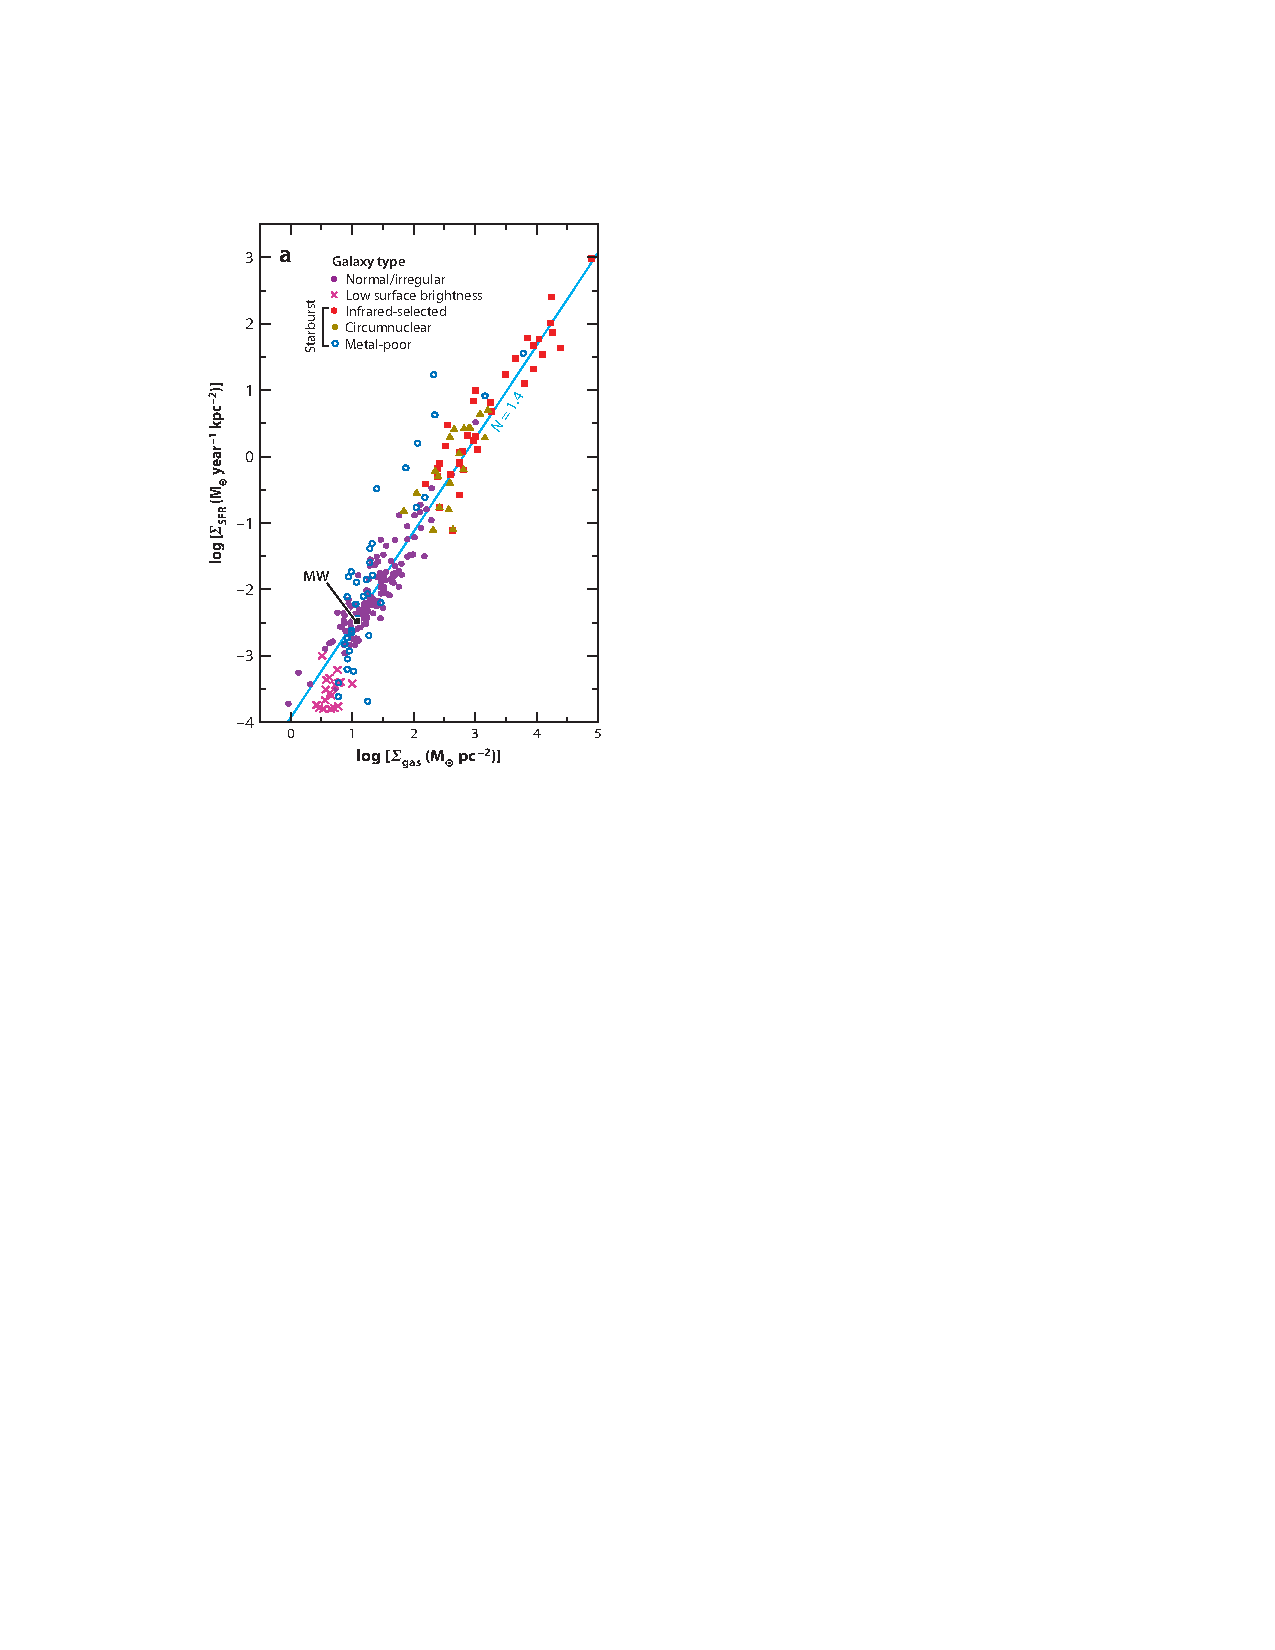
\includegraphics[width=\linewidth]{ksrelation_kennicutt12}
\caption[Whole-galaxy Kennicutt-Schmidt relation]{
\label{fig:ksrelation}
The observed collection between gas surface density $\Sigma_{\mathrm{gas}}$ and star formation surface density $\Sigma_{\mathrm{SFR}}$, integrating over whole galaxies. Galaxy classes are as indicated in the legend; circumnuclear indicates circumnuclear starburst, IR-selected is galaxies selected based on their high-infrared luminosity, metal-poor is galaxies with substantially sub-solar metallicity, and LSB is low surface-brightness galaxies. Data from \citet{kennicutt12a}.
}
\end{marginfigure}

\begin{equation}
\Sigma_{\rm SFR} \propto \Sigma_{\rm gas}^{1.4}.
\end{equation}

There are a few caveats to this. This fit uses the same value of $X_{\rm CO}$ for all galaxies, but there is excellent evidence that $X_{\rm CO}$ is lower for starbursts and higher for metal-poor galaxies. Correcting for this effect would tend to move the metal-poor galaxies that lie above the relation back toward it (by increasing their inferred $\Sigma_{\rm gas}$), while steepening the relation overall (by moving the galaxies with the highest star formation rates systematically to lower $\Sigma_{\rm gas}$). Correcting for this effect increases the slope from $\sim 1.4$ to something more like $\sim 1.7-1.8$ \citep[e.g.,][]{narayanan12a}, but with a significantly larger uncertainty. For extreme but not utterly implausible scalings of $X_{\rm CO}$ with star formation rate or gas content, one can get slopes as steep as $\sim 2$.

\begin{marginfigure}
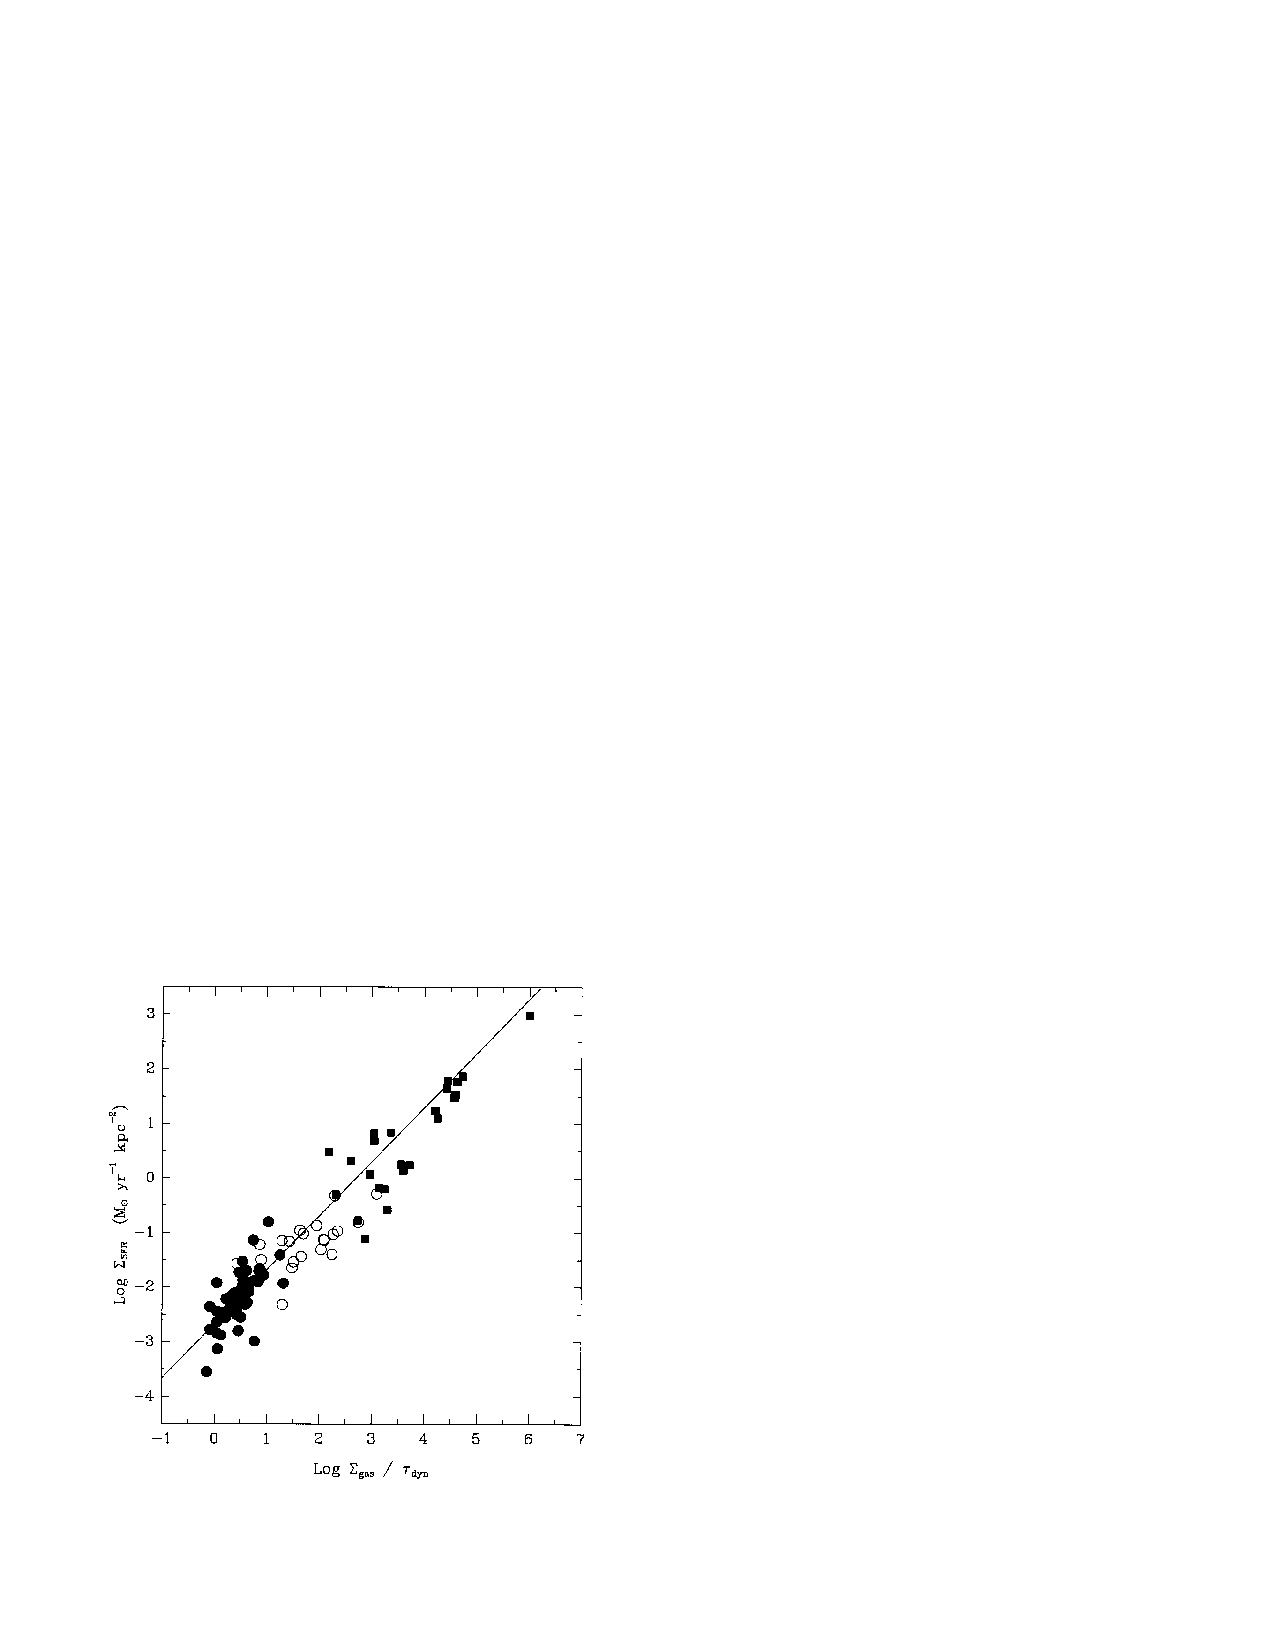
\includegraphics[width=\linewidth]{ksrelation_kennicutt98}
\caption[Whole-galaxy Kennicutt-Schmidt relation, including orbital time]{
\label{fig:ksrelation_torb}
The observed collection between gas surface density divided by galaxy orbital period $\Sigma_{\mathrm{gas}}/\tau_{\mathrm{dyn}}$ and star formation surface density $\Sigma_{\mathrm{SFR}}$, integrating over whole galaxies. Filed circles are normal disk galaxies, open circles are circumnuclear starbursts, and filled squares are starburst galaxies. Credit: \citet{kennicutt98a}, \copyright AAS. Reproduced with permission.
}
\end{marginfigure}

While this is one way of plotting the data, another way is to make use of the galactic rotation curve. The star formation rate per unit area has units of mass per unit time per unit area, so it is natural to compare this to the gas mass per unit area divided by the galactic orbital period $t_{\rm orb}$, which has the same units. Physically, this relationship describes what fraction of the gas mass is transformed into stars per orbital period. Making this plot yields a relationship that actually fits the data every bit as well as the $\Sigma_{\rm gas} - \Sigma_{\rm SFR}$ plot (Figure \ref{fig:ksrelation_torb}), and with a slope of unity, i.e., $\Sigma_{\rm SFR} \propto \Sigma_{\rm gas}/t_{\rm orb}$.

\subsection{High-Redshift Galaxies}

Since Kennicutt's initial collection, a number of other authors have added much more data to this plot, principally but not exclusively from the high redshift Universe. The expanded data set suggests that there isn't a single relationship between $\Sigma_{\rm gas}$ and $\Sigma_{\rm SFR}$, but that instead "normal galaxies" and "starbursts" occupy different loci on the $\Sigma_{\rm gas} - \Sigma_{\rm SFR}$ plane (Figure \ref{fig:sfsequences}).

This result should be taken with a considerable grain of salt. In part, the bimodality is exaggerated by the use of different $X_{\rm CO}$ factors for the two sequences, which spreads them further apart. If one uses a single $X_{\rm CO}$, the bimodality is far less clear. As mentioned above, there are excellent reasons to think that $X_{\rm CO}$ is not in fact constant, but conversely there are no good reasons to think that it is bimodal as opposed to changing continuously. A second issue is one of selection: the samples that occupy the two loci are selected in different ways, and this may well lead to an artificial bimodality that is not present in the real galaxy population.
\begin{marginfigure}
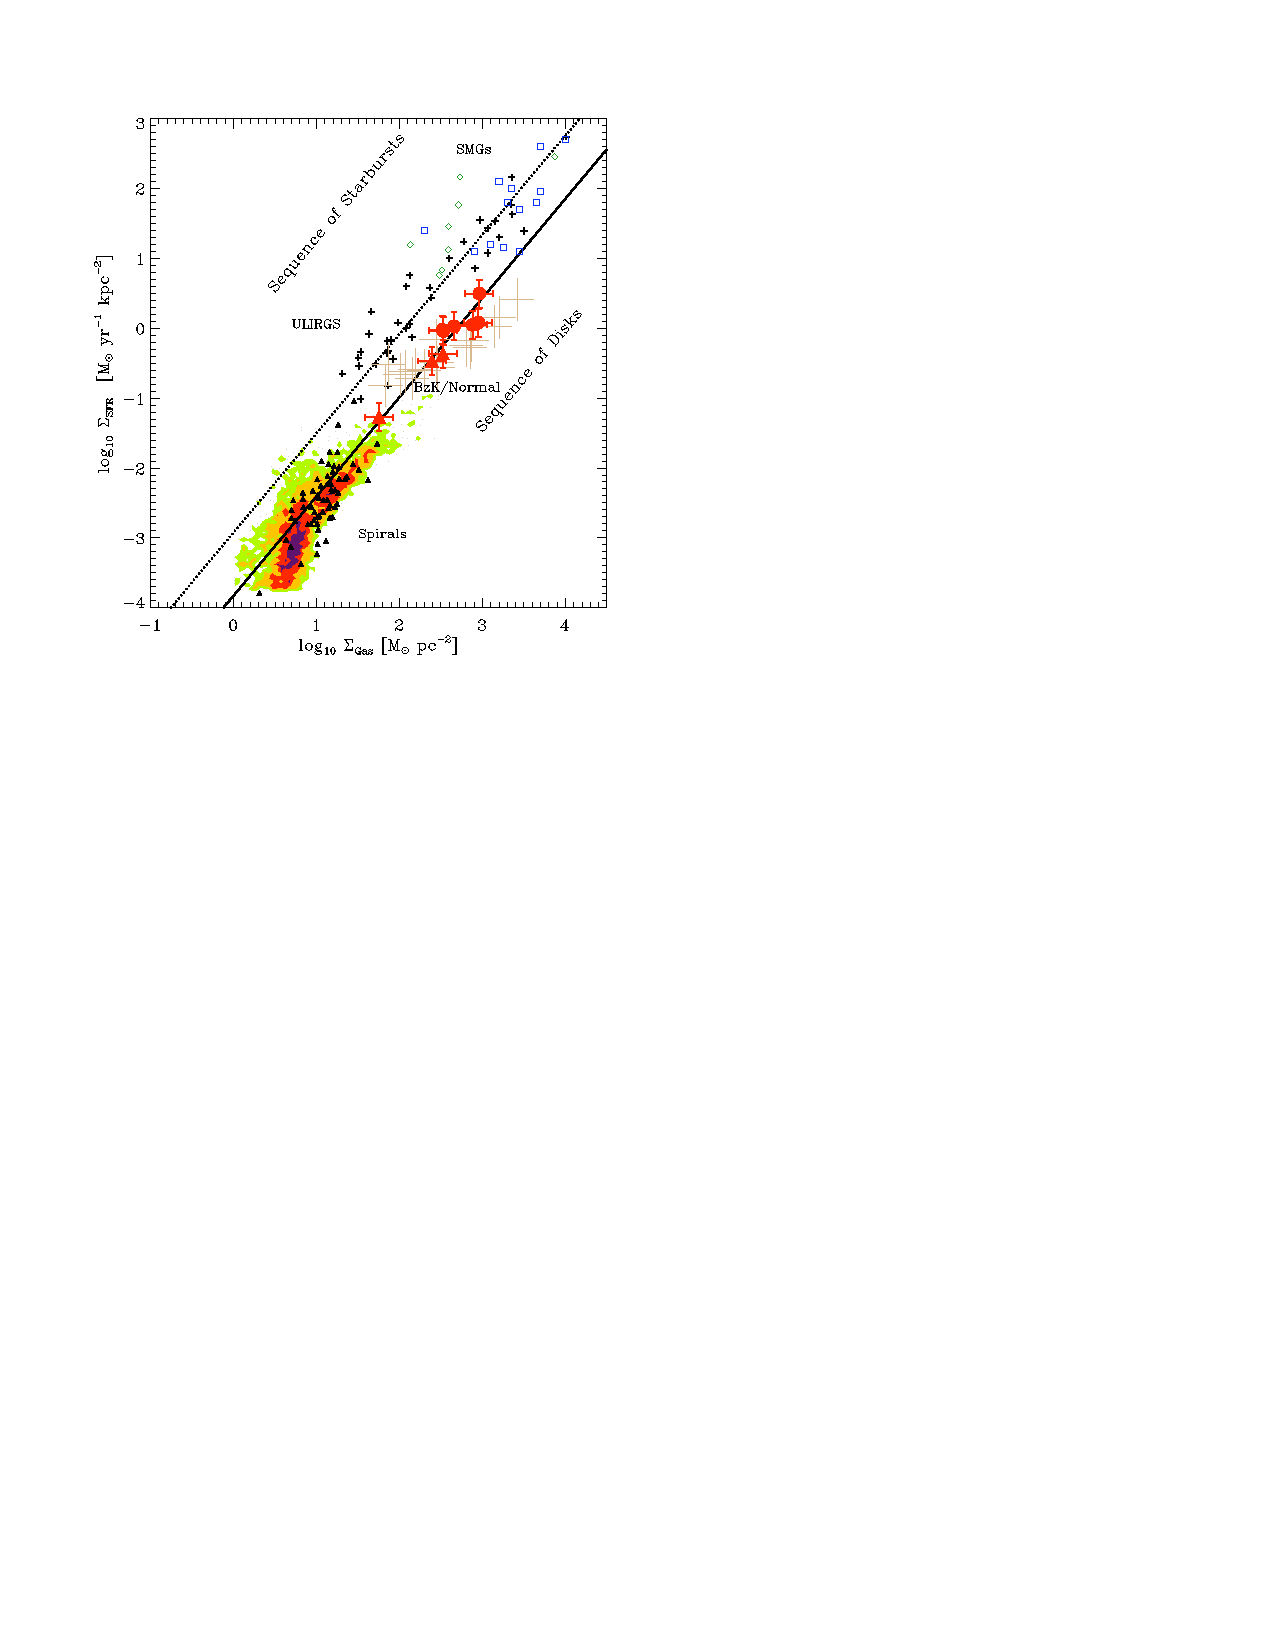
\includegraphics[width=\linewidth]{sfsequences_daddi10}
\caption[Kennicutt-Schmidt relation, with additional high-redshift data]{
\label{fig:sfsequences}
Kennicutt-Schmidt relation including an expanded high-redshift sample, with two proposed sequences (``disks" and ``starbursts") indicated. Points are integrated-galaxy measurements, while contours are spatially-resolved regions (see below). Credit: \citet{daddi10a}, \copyright AAS. Reproduced with permission.
}
\end{marginfigure}

Nonetheless, the point remains that it is far from clear that there is a single, uniform relationship between $\Sigma_{\rm gas}$ and $\Sigma_{\rm SFR}$. On the other hand, the $\Sigma_{\rm gas}/t_{\rm orb}$ versus $\Sigma_{\rm SFR}$ relationship appears to persist even in the expanded data set (Figure \ref{fig:sftorb}).
\begin{marginfigure}
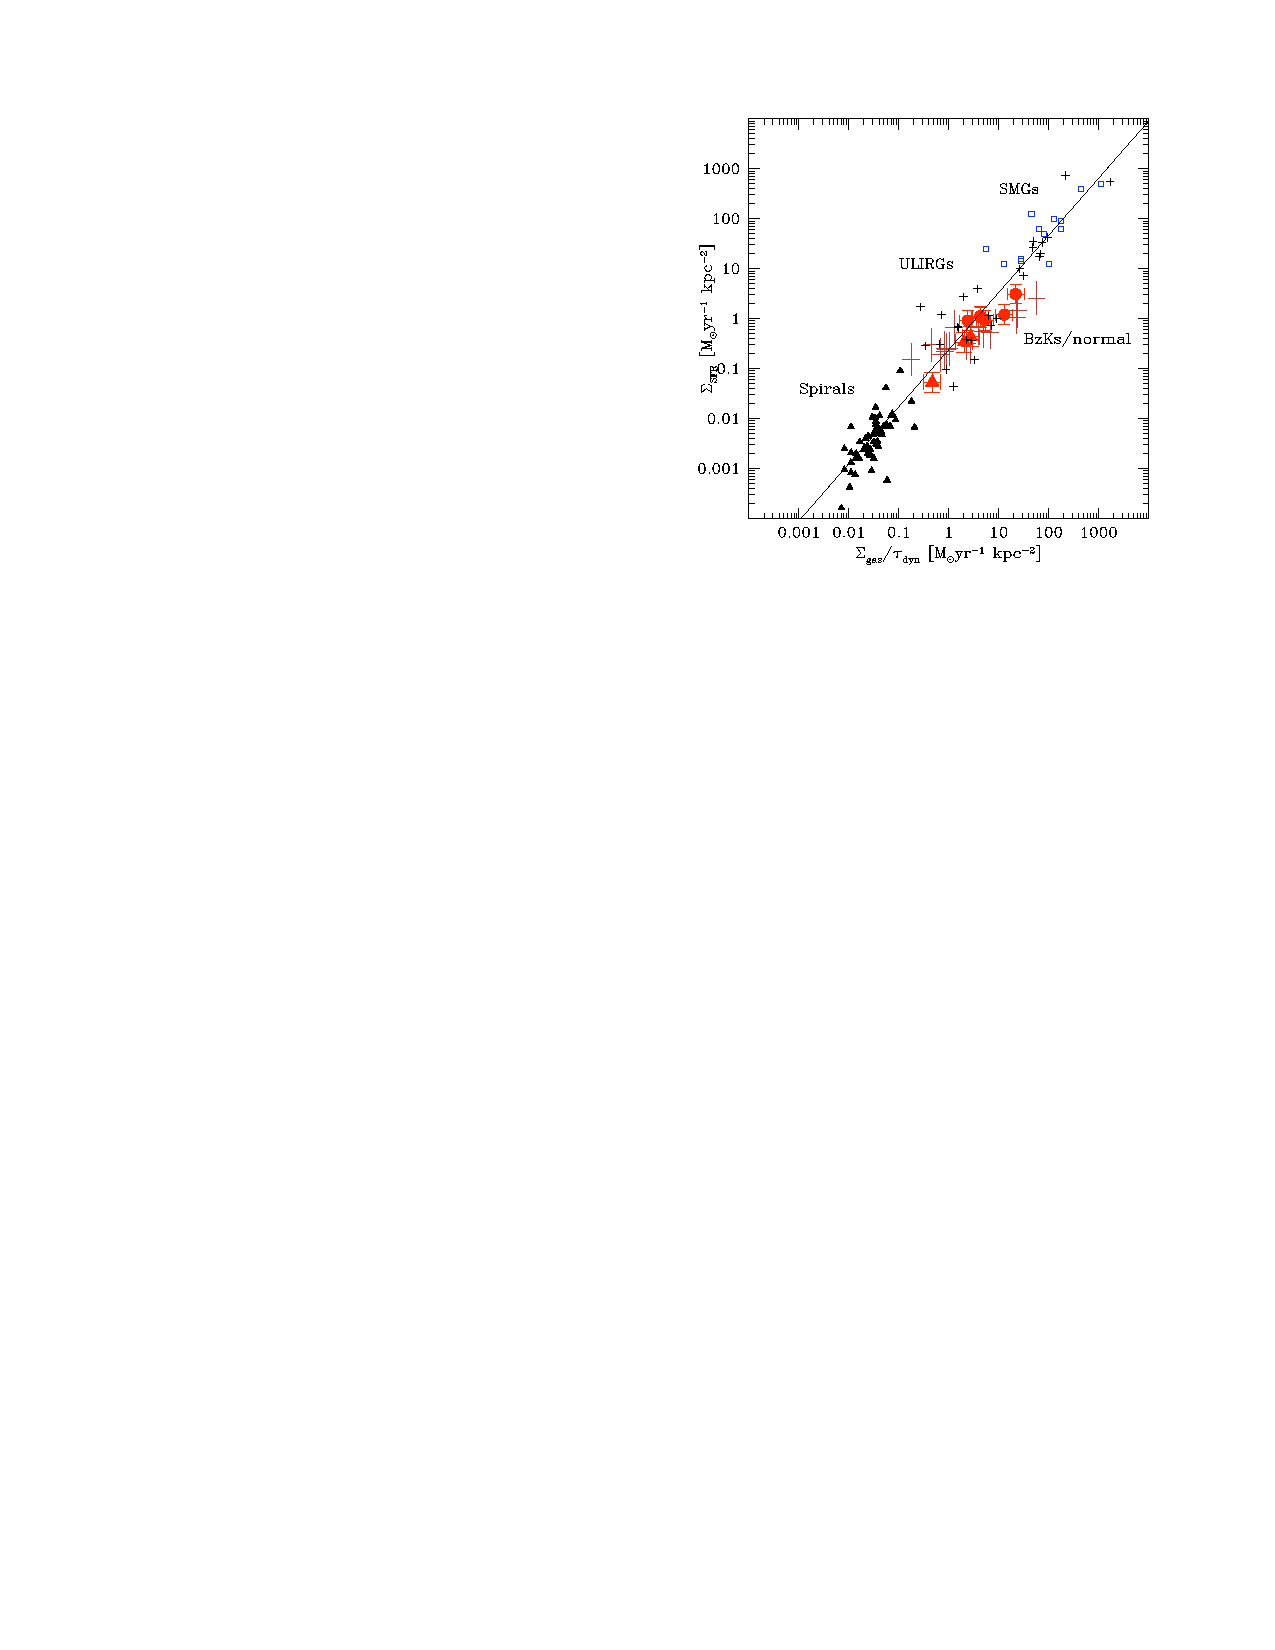
\includegraphics[width=\linewidth]{sftorb_daddi10}
\caption[Kennicutt-Schmidt relation, orbital time version, with additional high-redshift data]{
\label{fig:sftorb}
Kennicutt-Schmidt relation in its $\Sigma_{\rm SFR}-\Sigma_{\rm gas}/t_{\rm orb}$ form, including an expanded high-redshift sample. Points are the same as in Figure \ref{fig:sfsequences}, except that points for which the orbital time are unavailable have been omitted. Credit: \citet{daddi10a}, \copyright AAS. Reproduced with permission.
}
\end{marginfigure}

\subsection{Dwarfs and low surface brightness galaxies}

A second area in which Kennicutt's original sample has been greatly expanded is in the study of dwarf galaxies. There were a few dwarfs in Kennicutt's original sample, but not that many, due to the difficulty of measuring star formation rates in low luminosity systems. Kennicutt's original sample used star formation rates primarily based on H$\alpha$ and infrared, but these are difficult to use on dwarfs: the H$\alpha$ is faint and hard to pick out above the sky background due to the low overall star formation rate, and the IR is faint because dwarfs tend to have little dust and thus reprocess little of their starlight into the IR. The situation improved greatly with the launch of \textit{GALEX} in 2003, which allowed the study of dwarfs in the FUV. The FUV has the advantage that, from space, the background is nearly zero, and thus much lower levels of star formation activity can be detected much more easily.

Another problem that does remain for dwarfs is that the CO to H$_2$ conversion factor is almost certainly different than in spirals, and the CO is often so faint as to be undetectable. This makes it impossible to measure the molecular gas content of many dwarfs without using a better proxy like dust. Only with the launch of \textit{Herschel} has this been possible with even a modest sample of dwarfs; prior to that, with the exception of the Small Magellanic Cloud (which could be mapped in dust with \textit{IRAS} due to its large size on the sky). Nonetheless, the H~\textsc{i} can certainly be measured, and since the H~\textsc{i} almost certainly dominates the total gas, the relationship between total gas content and star formation could also be measured.

When the data are plotted, the result is that dwarfs generally lie below the linear extrapolation of the Kennicutt relationship when one considers their total gas content (Figure \ref{fig:ks_lsb}).

\section{The Spatially-Resolved Star Formation Rate}

\begin{marginfigure}
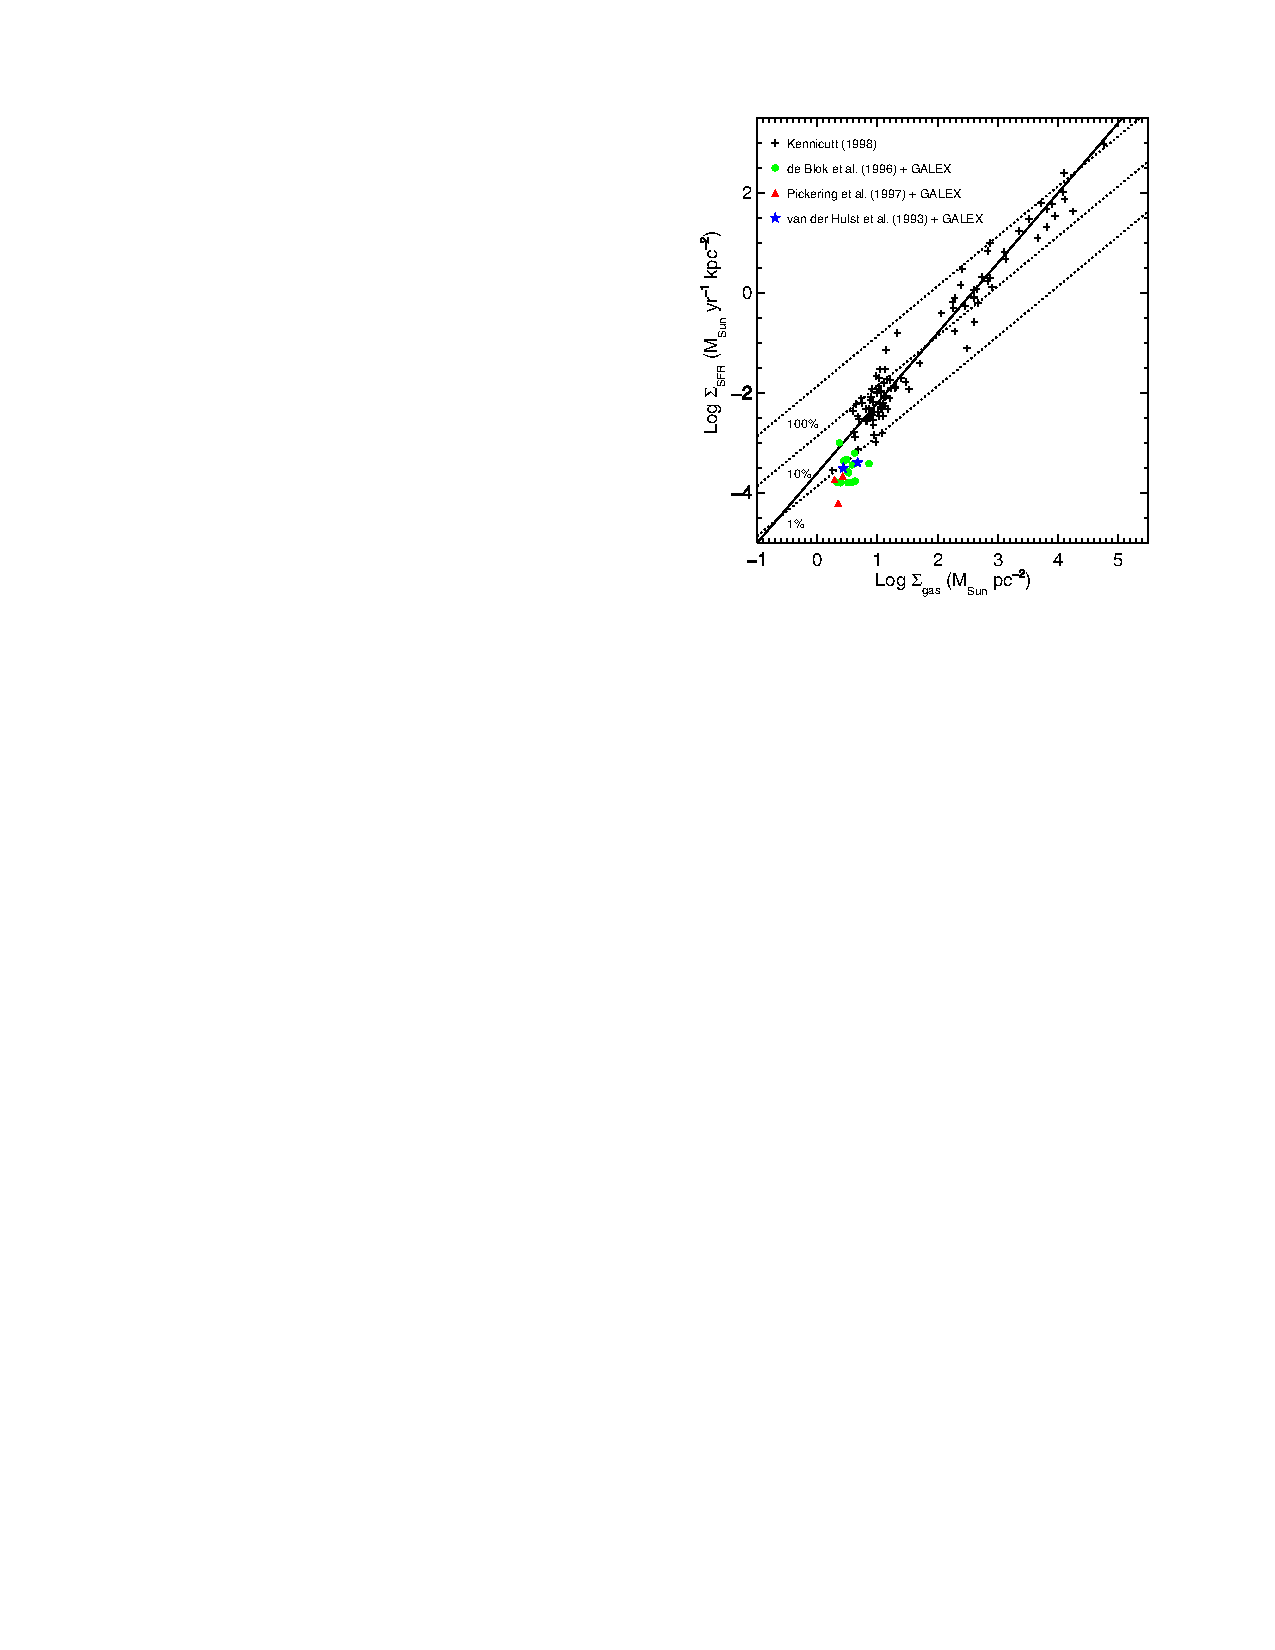
\includegraphics[width=\linewidth]{ks_lsb_wyder09}
\caption[Kennicutt-Schmidt relation, with additional low surface brightness sample]{
\label{fig:ks_lsb}
Kennicutt-Schmidt relation including an expanded sample of low surface brightness galaxies. The black points are the original \citet{kennicutt98a} sample, while the colored points are the low surface brightness sample. Credit: \citet{wyder09a}, \copyright AAS. Reproduced with permission.
}
\end{marginfigure}

The previous section summarizes the observational state of play as far as single points per galaxy goes, but what about if we start to resolve galaxies? Starting around 2006-7, instrumentation reached the point where it became possible to make spatially resolved maps of the gas and star formation in galaxies. For gas, the key development was the advent of heterodyne receiver arrays, which greatly increased mapping speed and made it possible to produce maps of the CO in nearby galaxies at resolutions of $\sim 1$ kpc or better in reasonable amounts of observing time. For star formation, the key was the development of space-based infrared telescopes, first \textit{Spitzer} and then \textit{Herschel}, that could make images of the dust-reprocessed light from a galactic disk. Armed with these new technologies, a number of groups began to make maps of the relationship between gas and star formation within the disks of nearby galaxies, starting at $\sim 1$ kpc or better scales and eventually going in some cases to $\sim 10$ pc scales.

\subsection{Relationship to Molecular Gas}

One of the first results to emerge from these studies was the strikingly-good correlation between molecular gas and star formation when both are measured at $\sim 0.5-1$ kpc scales (Figure \ref{fig:tdeph2_leroy13}). The correlation between molecular gas and star formation is noticeably tighter than the galaxy-averaged correlation first explored by Kennicutt. In nearby galaxies, at least in the inner disks where CO is bright enough to be detectable, there appears to be a roughly constant depletion time $t_{\rm dep} = \Sigma_{\rm H_2}/\Sigma_{\rm SFR} \approx 2$ Gyr. There is considerable debate about whether the depletion time is actually constant, or whether it increases or decreases slightly with $\Sigma_{\rm H_2}$. This debate mostly turns on technical questions of how to handle background subtraction and correct for contamination, and on how to properly fit a very noisy data set. Thus indices within a few tenths of $1.0$ for $\Sigma_{\rm SFR}$ versus $\Sigma_{\rm H_2}$ cannot be ruled out. Nonetheless, the correlation is clear and striking.

\begin{figure}
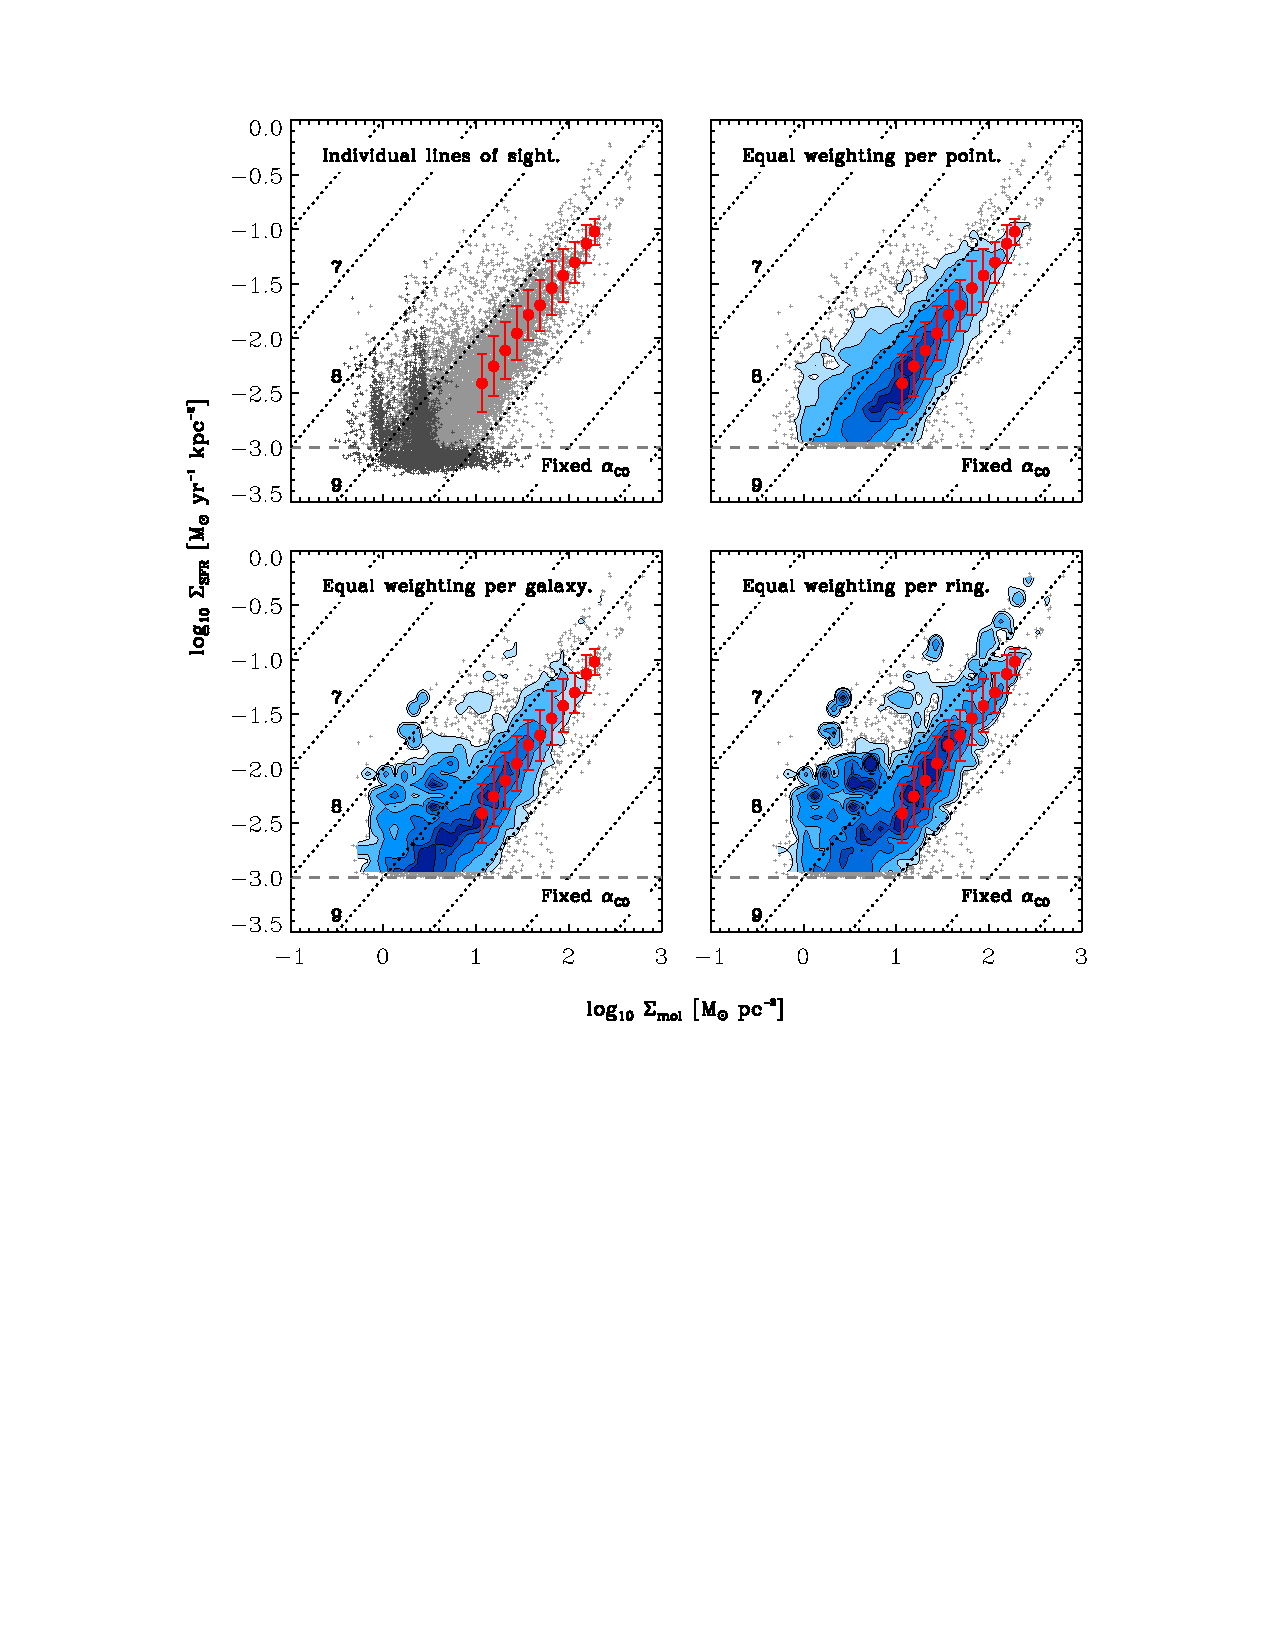
\includegraphics[width=\linewidth]{tdeph2_leroy13}
\caption[Kennicutt-Schmidt relation for galaxies resolved at $\sim$kpc scales]{
\label{fig:tdeph2_leroy13}
Kennicutt-Schmidt relation for $\sim$kpc-sized lines of sight through a sample of nearby galaxies, computed with fixed CO-H$_2$ conversion factor. The four panels show points individual lines of sight (top left), contours with equal weighting per line of sight (top right), contours with equal weighting per galaxy (bottom left) and contours with equal weighting per azimuthal ring (bottom right). Dotted lines of slope unity are lines of constant $t_{\mathrm{dep}} = \Sigma_{\mathrm{SFR}} / \Sigma_{\mathrm{mol}}$, with the number indicating the log of the depletion time in yr. Gray horizontal dashed lines mark the star formation rate sensitivity limit. Credit: \citet{leroy13a}, \copyright AAS. Reproduced with permission.
}
\end{figure}

Also striking is the extent to which this depletion time is \textit{in}sensitive to any other properties of the galaxy.  Varying the stellar surface density or the local orbital timescale, or the dust to gas ratio (once a dust to gas-dependent $X_{\rm CO}$ factor has been used) appears to have no significant effect on the star formation rate per unit molecular gas mass. Note that the lack of dependence on the orbital time scale is in striking contrast to the results for whole galaxy star formation rates, where plotting things in terms of surface density does not yield a single, simple sequence, but plotting in terms of surface density normalized by orbital time does.

How does this compare to the free-fall time in these clouds, which is the natural times scale on which they evolve? We have no direct access to the volume densities in these clouds, so we cannot answer the question directly. However, \citet{krumholz12a} suggest a simple \textit{ansatz} to estimate free-fall times. The idea was to exploit the fact that observed GMCs seem to have surface densities of $\sim 100$ $M_\odot$ pc$^{-2}$ in normal galaxies. They also have characteristic masses comparable to the Jeans mass in a thin slab of material,
\begin{equation}
M_{\rm GMC} = \frac{\sigma^4}{G^2 \Sigma_{\rm tot}},
\end{equation}
where $\sigma$ is the galactic velocity dispersion and $\Sigma_{\rm tot}$ is the total gas surface density. From a total mass and a surface density, one can compute a mean density and a corresponding free-fall time:
\begin{equation}
\rho_{\rm GMC} = \frac{3\sqrt{\pi}}{4} \frac{G \sqrt{\Sigma_{\rm GMC}^3 \Sigma_{\rm tot}}}{\sigma^2}.
\end{equation}
This must break down once the mean density at the mid-plane of the galaxy rises too high, as it must in some galaxies where the total gas surface density is $\gg 100$ $M_\odot$ pc$^{-2}$. To be precise, the mid-plane pressure in a galactic disk can be written
\begin{equation}
P = \rho \sigma^2 = \frac{\pi}{2} \phi_P G \Sigma_{\rm tot}^2,
\end{equation}
where $\phi_P$ is a constant of order unity that depends on the ratio of gas to stellar mass. For a pure gas disk, in the diffuse matter class we have shown that $\phi_P = 1$, but realistic values in actual galaxy disks are $\sim 3$. Combining these statements, we obtain
\begin{equation}
\rho_{\rm mp} = \frac{\pi \phi_P G \Sigma_{\rm tot}^2}{2\sigma^2}.
\end{equation}
The simple approximation suggested by \citeauthor{krumholz12a} is just to use the larger of $\rho_{\rm GMC}$ and $\rho_{\rm mp}$. If one does so, then it becomes possible to estimate $t_{\rm ff}$ from observable quantities. The result of this exercise is that the observed depletion times seen in external galaxies are generally consistent with $\epsilon_{\rm ff} \approx 0.01$, with a scatter of about a factor of 3. The same is true if we put the whole-galaxy points on the plot, although for them the uncertainties are considerably greater (Figure \ref{fig:ks_krumholz14}).

\begin{figure}
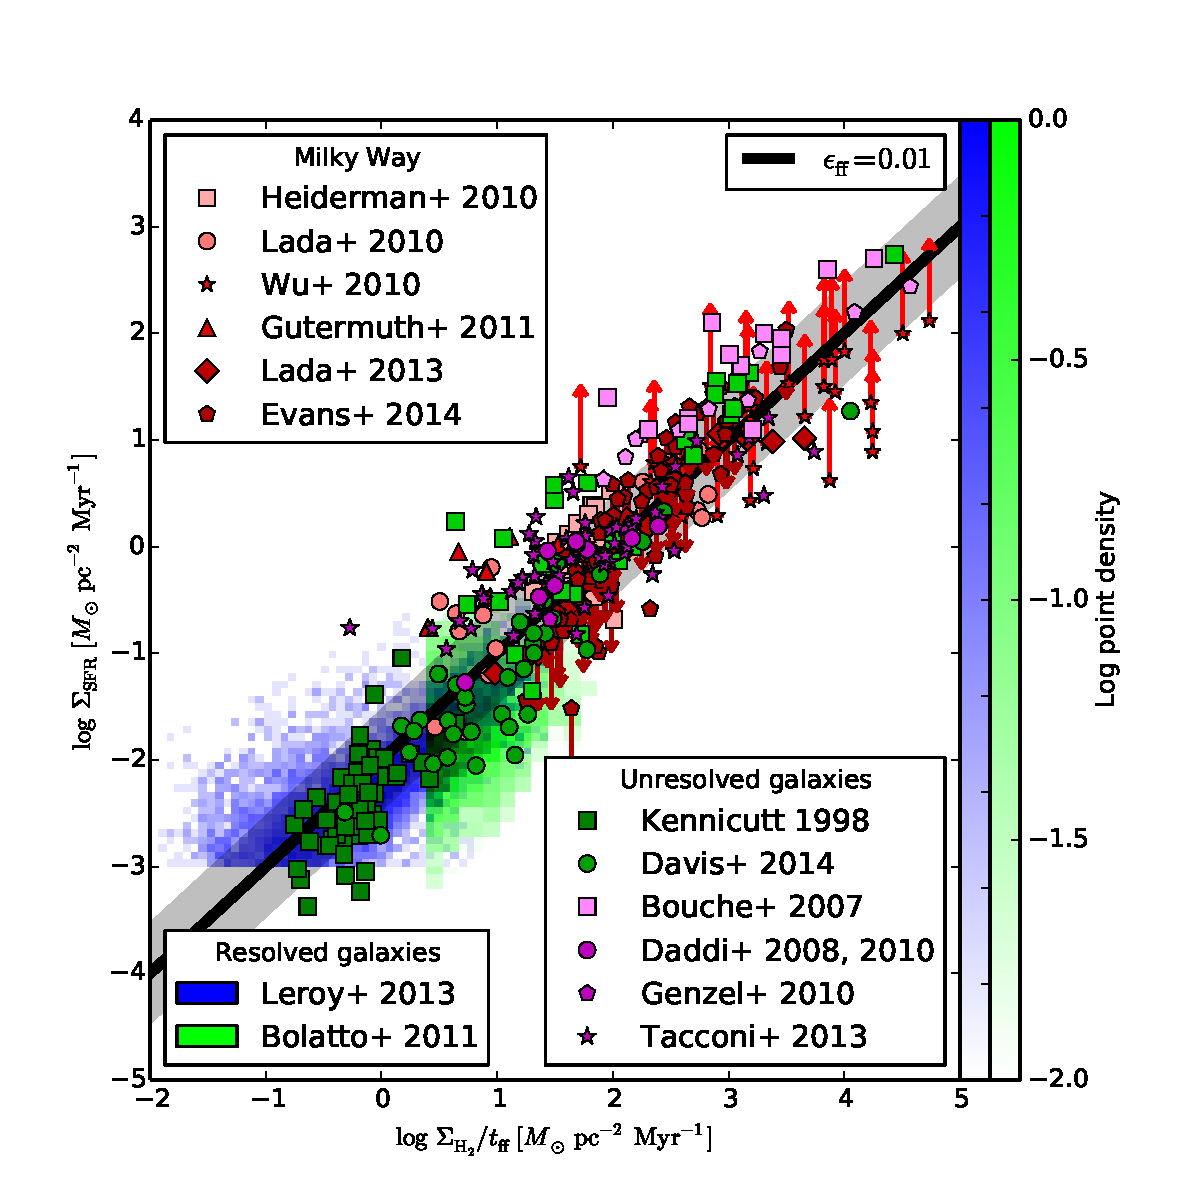
\includegraphics[width=\linewidth]{eff_krumholz14}
\caption[Kennicutt-Schmidt relation normalized by the free-fall time]{
\label{fig:ks_krumholz14}
Kennicutt-Schmidt relation normalized by the estimated free-fall time. Points plotted include resolved pixels in nearby galaxies (blue and green rasters), unresolved galaxies at low (green) and high (purple) redshift, and individual clouds within the Milky Way (red). Reprinted from Phys. Rep., 539, \citeauthor{krumholz14c}, "The big problems in star formation: The star formation rate, stellar clustering, and the initial mass function", 49-134, 2014, with permission from Elsevier.
}
\end{figure}

Finally, some important caveats are in order. First, this result is limited to the inner parts of galaxies where there is significant CO emission. In outer disks where there is little molecular gas and CO is faint, molecular emission can be detected only by stacking entire rings or focusing on local patches of strong emission, so the sort of pixel-by-pixel unbiased analysis done for inner galaxies is not yet possible. Second, this sample covers a very limited range of galaxy properties, certainly compared to the high-$z$ data. The pixel by pixel analysis can only be done for a large sample of local galaxies, within $\sim 20$ Mpc, and this volume does not contain any of the starbursts that form the upper part of the sequences seen in the local Kennicutt or high-$z$ samples.

A third and final caveat has to do with scale-dependence. Depending on the scales over which one averages, the correlation between molecular gas and star formation can be better or worse. Generally speaking, as one goes to smaller and smaller scales, the scatter in the $\Sigma_{\rm H_2} - \Sigma_{\rm SFR}$ correlation increases, and systematic biases start to appear. If one focuses on peaks of the H$_2$ distribution, one obtains systematically longer depletion times than for similar apertures centered on peaks of the inferred star formation rate distribution. Figure \ref{fig:ksscale_schruba10} illustrates the observational situation.
\begin{marginfigure}
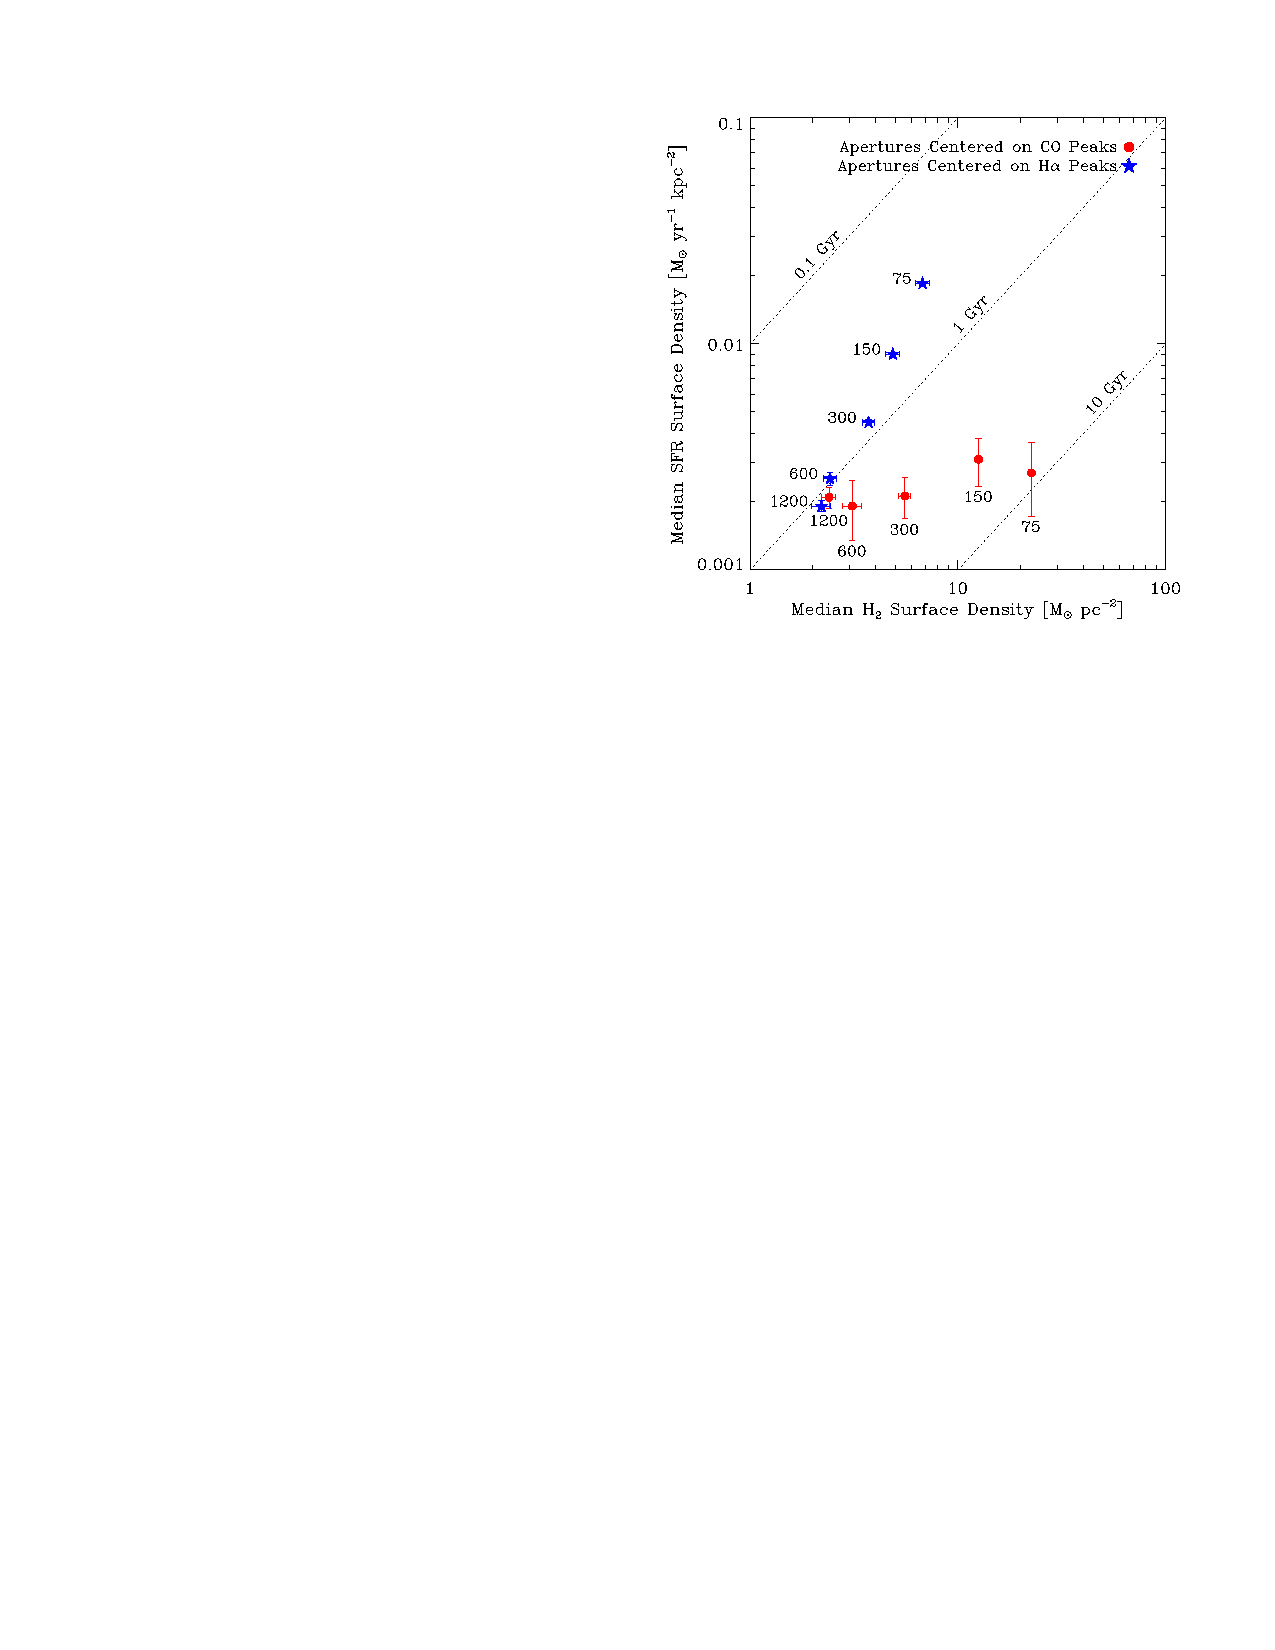
\includegraphics[width=\linewidth]{ksscale_schruba10}
\caption[Kennicutt-Schmidt relation averaged on different size scales in M33]{
\label{fig:ksscale_schruba10}
Kennicutt-Schmidt relation on different size scales. The points show the median surface densities of gas and star formation, using apertures of $75-1200$ pc in size, centered in CO peaks (red) and H$\alpha$ peaks (blue). Dotted lines of slope unity are lines of constant $t_{\mathrm{dep}} = \Sigma_{\mathrm{SFR}} / \Sigma_{\mathrm{mol}}$, with the number indicating the depletion time. Credit: \citet{schruba10a}, \copyright AAS. Reproduced with permission.
}
\end{marginfigure}

The most likely explanation for this is that, on sufficiently small scales, the central assumption that we are looking at an "average" piece of a galaxy begins to break down. If we focus on peaks of the H$_2$ distribution, we are looking at places where molecular gas is just now accumulating and there has not yet been time for much star formation to take place. In terms of the classification scheme discussed in Chapter \ref{ch:gmcs}, these represent class I clouds. If we focus on peaks in the H$\alpha$ distribution (the usual proxy for star formation rate in this sort of study), we are looking at H~\textsc{ii} regions where a molecular cloud once was, and which has since mostly been dispersed. In terms of the molecular cloud types discussed in Chapter \ref{ch:gmcs}, these are class III clouds.

In this case our proxies are misleading -- the CO tells us about the instantaneous amount of molecular gas present, while the H$\alpha$ tells us about the average number of stars formed over the last $\sim 5$ Myr, and those are not exactly what we want to compare. We want either to compare the instantaneous molecular mass and star formation rate, or the averages of both molecular mass and star formation rate over similar timescales. If we average over a large enough piece of the galaxy, our beam encompasses clouds in all stages of evolution, so we get a representative average, but that ceases to be true as we go to smaller and smaller scales. Indeed, the characteristic scale at which that ceases to be true can be used as something of a proxy for characteristic molecular cloud lifetime, a point made recently by \citet{kruijssen14c}.


\subsection{Relationship to Atomic Gas and All Neutral Gas}

The results for molecular gas are in striking contrast to the results for total gas or just atomic gas. If one considers only atomic gas, one finds that the H~\textsc{i} surface density reaches a maximum value which it does not exceed, and that the star formation rate is essentially uncorrelated with the H~\textsc{i} surface density when it is at this maximum (Figure \ref{fig:kshi_bigiel08}). In the inner parts of galaxies, star formation does not appear to care about H~\textsc{i}.
\begin{marginfigure}
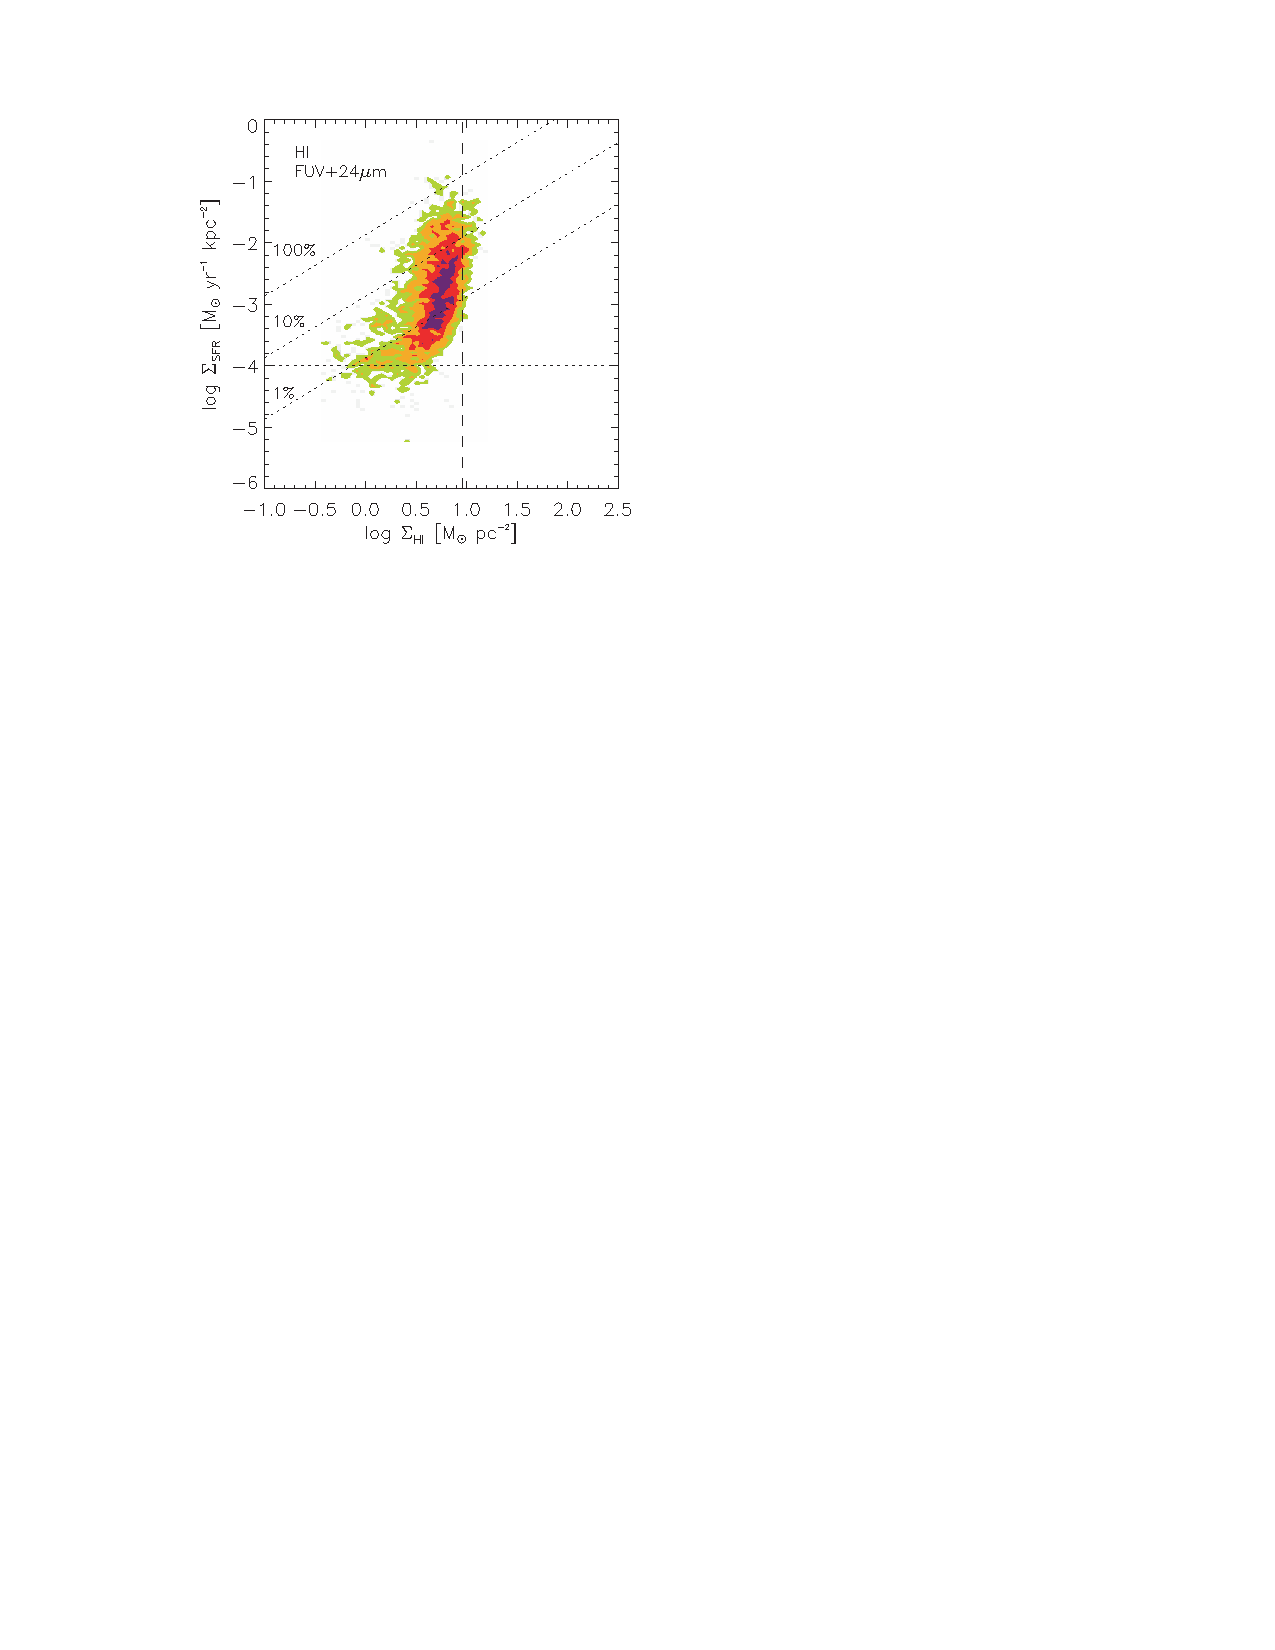
\includegraphics[width=\linewidth]{kshi_bigiel08}
\caption[Kennicutt-Schmidt relation for H~\textsc{i} gas in inner galaxies]{
\label{fig:kshi_bigiel08}
Kennicutt-Schmidt relation for H~\textsc{i} gas in inner galaxies, averaged on $\sim 750$ pc scales. Contours indicate the density of points. Credit: \citet{bigiel08a}, \copyright AAS. Reproduced with permission.
}
\end{marginfigure}

On the other hand, if one considers the outer parts of galaxies, there is a correlation between H~\textsc{i} content and star formation, albeit with a very, very large scatter (Figure \ref{fig:kshi_bigiel10}). While there is a correlation, the depletion time is extremely long -- typically $\sim 100$ Gyr. It is important to point out that, while it is not generally possible to detect CO emission over broad areas in these outer disks, when one stacks the data, the result is that the depletion time in molecular gas is still $\sim 2$ Gyr. Thus these very long depletion times appear to be a reflection of a very low H$_2$ to H~\textsc{i} ratio, but one that does not go all the way to zero, and instead stops at a floor of $\sim 1-2\%$.

\begin{figure}
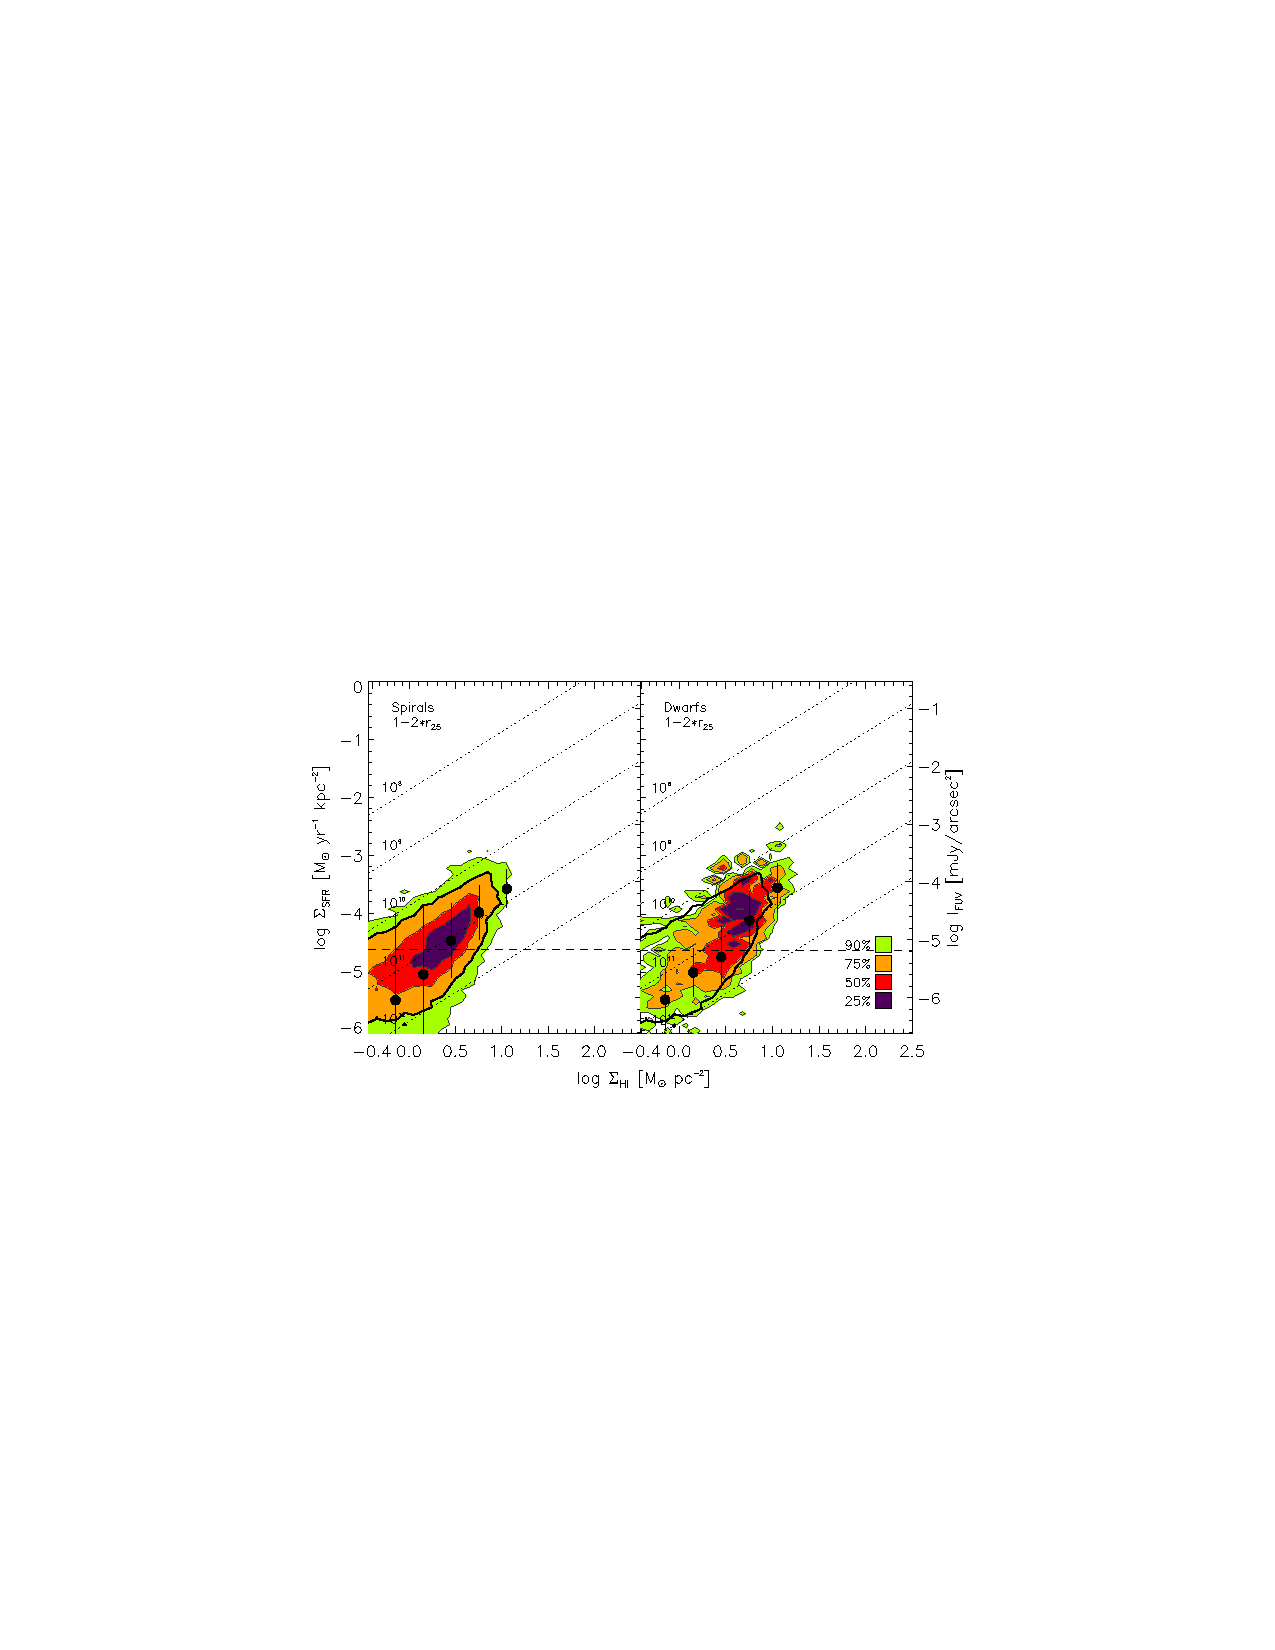
\includegraphics[width=\linewidth]{kshi_bigiel10}
\caption[Kennicutt-Schmidt relation for H~\textsc{i} gas in outer galaxies]{
\label{fig:kshi_bigiel10}
Kennicutt-Schmidt relation for H~\textsc{i} gas in outer galaxies, averaged on $\sim 750$ pc scales. Contours indicate the density of points, and the two panels are for spirals and dwarfs, respectively. Black points with error bars indicate the mean and dispersion in bins of $\Sigma_{\mathrm{HI}}$. Credit: \citet{bigiel10a}, \copyright AAS. Reproduced with permission.
}
\end{figure}

If instead of plotting just atomic or molecular gas on the $x$-axis, one plots total gas, then a clear relationship emerges. At high gas surface density, the ISM is mostly H$_2$, and this gas forms stars with a constant depletion time of $\sim 2$ Gyr. In this regime, the H~\textsc{i} surface density saturates at $\sim 10$ $M_\odot$ pc$^{-2}$, and has no relationship to the star formation rate. This constant depletion time begins to change at a total surface density of $\sim 10$ $M_\odot$ pc$^{-2}$, at which point the ISM begins to transition from H$_2$-dominated to H~\textsc{i}-dominated. Below this critical surface density, the star formation rate drops precipitously, and the depletion time increases by a factor of $\sim 50$ over a very small range in total gas surface density. Finally, below $\sim 10$ $M_\odot$ pc$^{-2}$, the star formation rate does correlate with both the total and H~\textsc{i} surface densities (which are roughly the same), but the depletion time is extremely long, and there is an extremely large amount of scatter. Figure \ref{fig:kstot_krumholz14} summarizes the data.

\begin{figure}
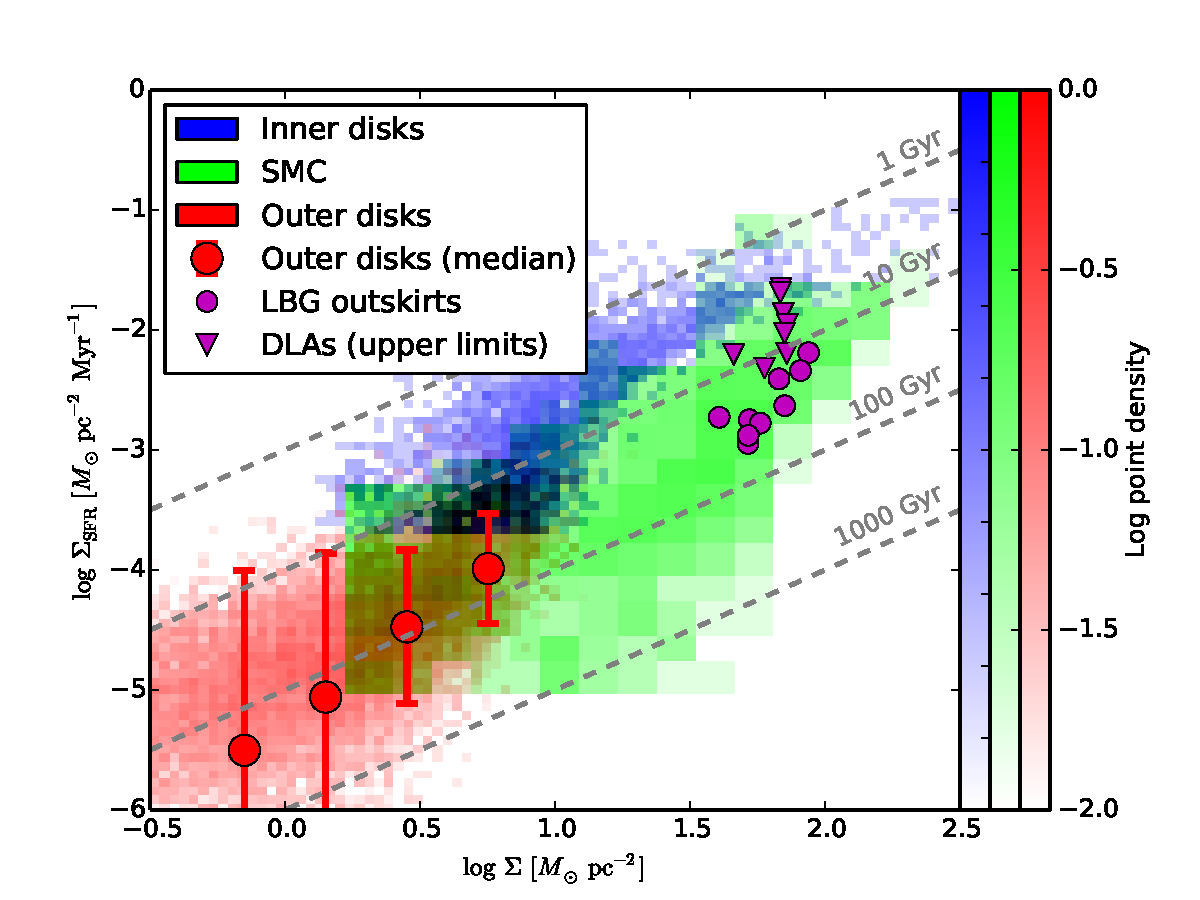
\includegraphics[width=\linewidth]{kstot_krumholz14}
\caption[Kennicutt-Schmidt relation for total gas in resolved galaxies]{
\label{fig:kstot_krumholz14}
Kennicutt-Schmidt relation for all gas, atomic plus molecular. The rasters show lines of sight through inner and outer galaxies and through the Small Magellanic Cloud, as indicated. Purple points indicate individual lines of sight through high-redshift systems, where H~\textsc{i} columns are measured in Ly$\alpha$ absorption. Reprinted from Phys. Rep., 539, \citeauthor{krumholz14c}, "The big problems in star formation: The star formation rate, stellar clustering, and the initial mass function", 49-134, 2014, with permission from Elsevier.
}
\end{figure}


\subsection{Additional Parameters}

In the H$_2$-dominated regime, as we have seen nothing seems to affect the star formation rate per unit molecular mass. However, that is not the case in the H~\textsc{i}-dominated regime, where the scatter is large and "second parameters" seem to have an effect. This regime is not understood very well, and the data are still incomplete, but two striking correlations are apparent in the data. First, in the H~\textsc{i}-dominated regime, the metallicity of the gas seems to matter. This is obvious is we compare the Small Magellanic Cloud, at metallicity 20\% of Solar, damped Lyman $\alpha$ systems (which have $\sim 10\%$ of Solar metallicity), and other low-metallicity dwarf galaxies (Figure \ref{fig:kstot_krumholz14}) to the bulk of the sample, which has near Solar metallicity. Indeed, the main effect of a low metallicity seems to be that the characteristic value of $\sim 10$ $M_\odot$ pc$^{-2}$ at which the gas goes from H~\textsc{i}- to H$_2$-dominated is shifted to higher surface densities.

Another parameter that appears to matter is the stellar surface density. Higher stellar surface densities appear to yield higher H$_2$ fractions and higher star formation rates at fixed gas surface density in the H~\textsc{i}-dominated regime. This correlation appears to be on top of the correlation with metallicity. Similarly, galactocentric radius seems to matter. Since all of these quantities are correlated with one another, it is hard to know what the driving factor(s) are.

\section{Star Formation in Dense Gas}

\subsection{Alternatives to CO}

The far all the observations we have discussed have used CO (or, in a few cases, dust emission) as the proxy of choice for H$_2$. This is by far the largest and richest data set available right now. However, it is of great interest to consider other tracers as well, in particular tracers of gas at higher densities. Doing so makes it possible, in principle, to map out the density distribution within the gas in another galaxy, and thereby to gain insight into how gas at different densities is correlated with star formation.

Moving past H$_2$, the next-brightest molecular line (not counting isotopologues of CO, which are generally found under the same conditions) in most galaxies is HCN. Other bright molecules are HCO$^+$, CS, and HNC, but we will focus on HCN as a synecdoche for all of these tracers. Like CO, the HCN molecule has rotational transitions that can be excited at low temperatures, and is abundant because it combines some of the most abundant elements. Thus the data set for correlations of HCN with star formation is the second-largest after CO. However, it is important to realize that this data set is still quite limited, and biased toward starburst galaxies where the HCN/CO ratio is highest. In normal galaxies HCN is $\sim 10$ times dimmer than CO, leading to $\sim 100\times$ larger mapping times in order to reach the same signal to noise. As a result, we are with HCN today roughly where we were with CO back in the time of \citet{kennicutt98a}, though that is starting to change.

Before diving into the data, let us pause for a moment to compare CO and HCN. The first few excited rotational states of CO lie 5.5, 16.6, 33.3, and 55.4 K above ground; the corresponding figures for HCN are 4.3, 12.8, 25.6, and 42.7 K. Thus the temperature ranges probed are quite similar, and all lines are relatively easy to excite at the temperatures typically found in molecular clouds. For CO, the collisional de-excitation rate coefficient for the $1-0$ transition is $k_{10} = 3.3\times 10^{-11}$ cm$^3$ s$^{-1}$ (at 10 K, for pure para-H$_2$ for simplicity), and the Einstein $A$ for the same transition is $A_{10} = 7.2\times 10^{-8}$ s$^{-1}$, giving a critical density
\begin{equation}
n_{\rm crit} = \frac{A_{10}}{k_{10}} = 2200\mbox{ cm}^{-3}.
\end{equation}
As discussed in Chapter \ref{ch:obscold}, radiative transfer effects lower the effective critical density significantly. In contrast, the collisional de-excitation rate coefficient and Einstein $A$ for HCN $1-0$ are $k_{10} = 2.4\times 10^{-11}$ cm$^3$ s$^{-1}$ and $A_{10}=2.4\times 10^{-5}$ s$^{-1}$, giving $n_{\rm crit} = 1.0\times 10^6$ cm$^{-3}$. Again, this is lowered somewhat by optical depth effects, but there is nonetheless a large contrast with CO. In effect, CO emission switches from rising quadratically with density to rising linearly with density at much lower volume density than does HCN, and thus HCN emission is considerably more weighted to denser gas. For this reason, HCN is often thought of as a tracer of the "dense" gas in galaxies.

\subsection{Correlations}

The first large survey of HCN emission from galaxies was undertaken by \citet{gao04b, gao04a}. This study had no spatial resolution -- it was simply one beam per galaxy. They found that, while CO luminosity measured in the same one-beam-per-galaxy fashion was correlated non-linearly with infrared emission (which was the proxy for star formation used in this study), HCN emission in contrast correlated almost linearly with IR emission. \citet{wu05a} showed that individual star-forming clumps in the Milky Way fell on the same linear correlation as the extragalactic observations.

This linear correlation was at first taken to be a sign that the HCN-emitting gas was the "dense" gas that was actively star-forming. In this picture, the high rates of star formation found in starburst galaxies are associated with the fact that they have high "dense" gas fractions, as diagnosed by high HCN to CO ratios. More recent studies, however, have shown that the correlation is not as linear as the initial studies suggested. Partly this is a matter of technical corrections to the existing data (e.g., observations that covered more of the disk of a galaxy), partly a matter of obtaining more spatially-resolved data (as opposed to one beam per galaxy), and partly a matter of expanded samples. Figure \ref{fig:hcn-ir} shows a recent compilation from \citet{usero15a}.

\begin{figure}
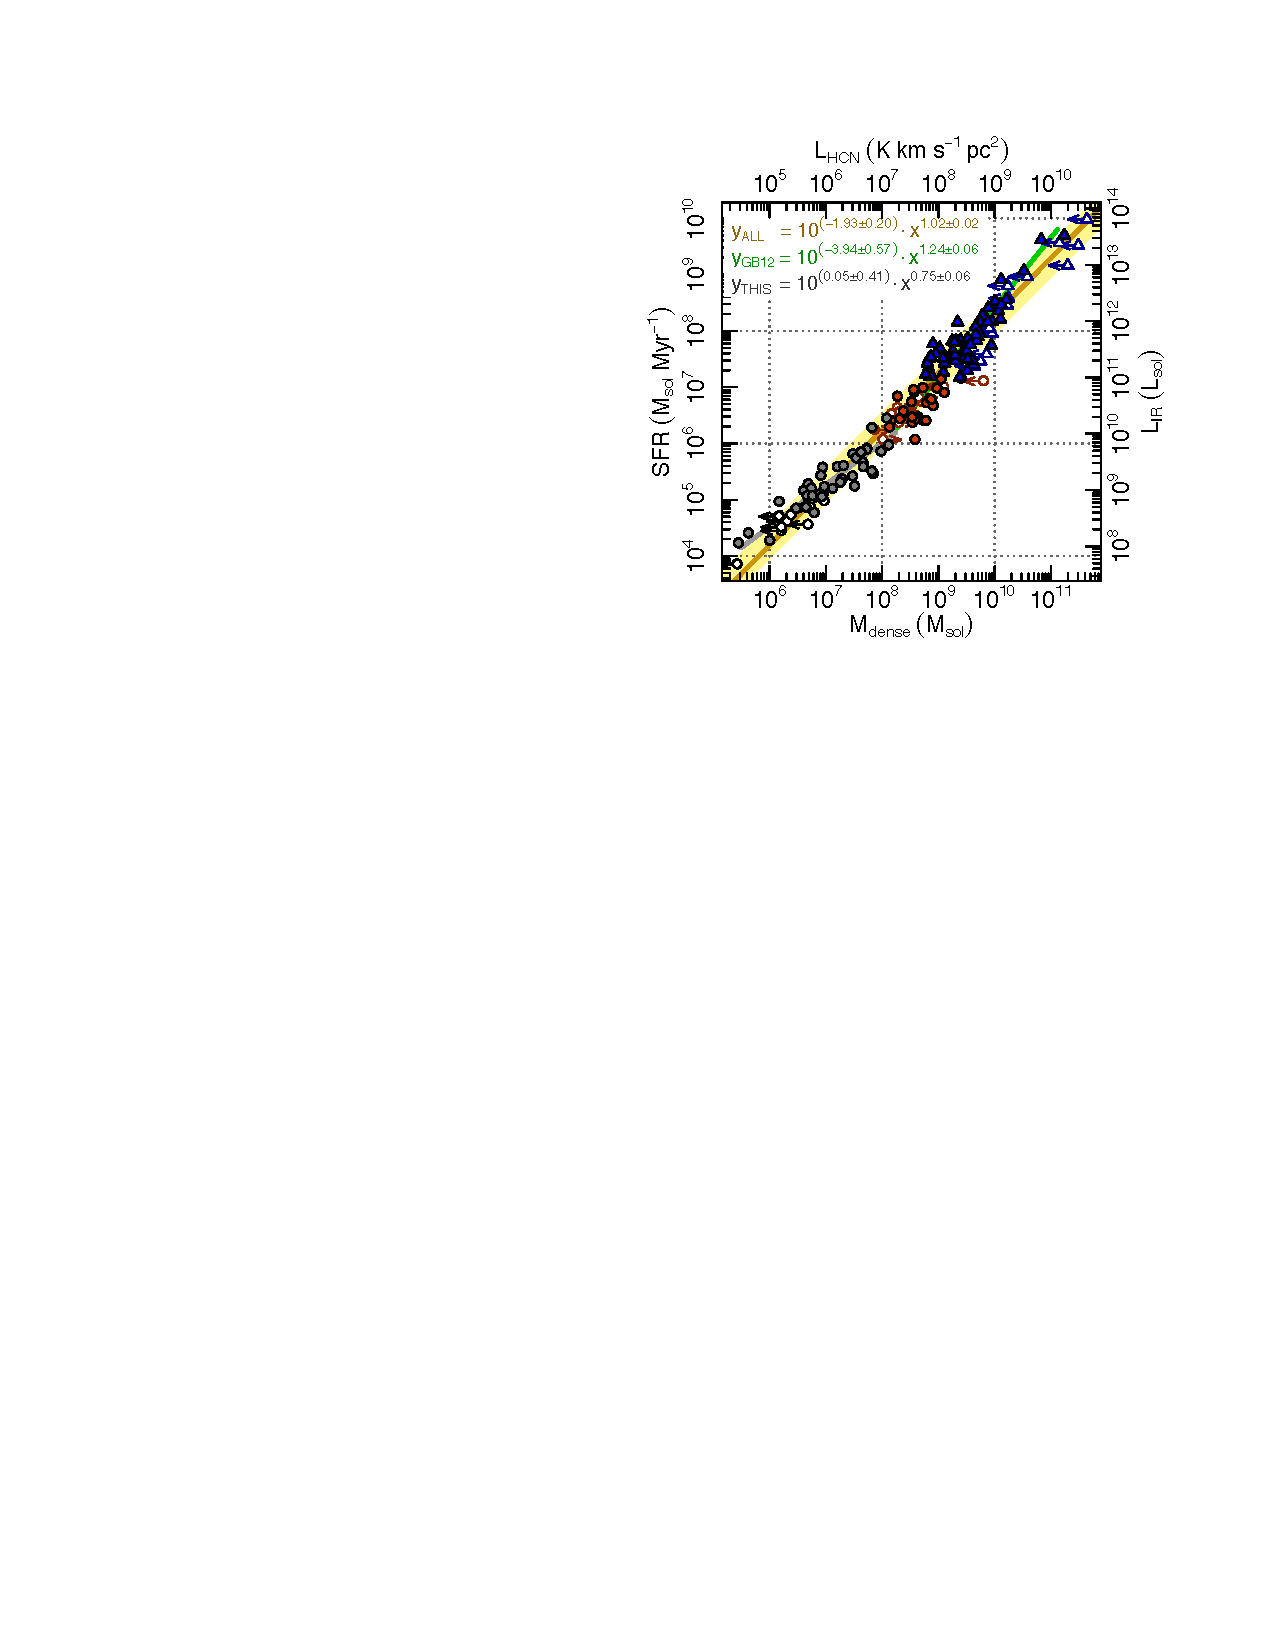
\includegraphics[width=\linewidth]{hcn-ir_usero15}
\caption[Infrared-HCN luminosity correlation]{
\label{fig:hcn-ir}
Observed correlation between HCN luminosity (converted to a mass of "dense" gas using an $X$ factor) and infrared luminosity (converted to a star formation rate). Gray points show resolved observations within galaxy disks, while red and blue points show unresolved observations of entire galaxy disks. Open points indicate upper limits. Credit: \citet{usero15a}, \copyright AAS. Reproduced with permission.
}
\end{figure}

Despite these revisions, it is clear that there is a generic trend that HCN and other tracers that have higher critical densities have a correlation with star formation that is flatter than for lower critical density tracers -- that is, a power law fit of the form
\begin{equation}
L_{\rm IR} \propto L_{\rm line}^p
\end{equation}
will recover an index $p$ that is closer to unity for higher critical density lines and further from unity for lower critical density ones. This has now been seen not just between HCN and CO, but also with higher $J$ lines of CO, and with HCO$^+$, another fairly bright line for which large enough data sets exist to make correlations.

\subsection{Physical Interpretation and Depletion Times}

To go beyond the sheer correlations, one must attempt to convert the observed quantities into physical ones. For infrared emission, this is straightforward: the galaxies where we have dense gas tracers are almost exclusively ones with high star formation rates, gas surface densities, and dust content. For them it is safe to assume that the great majority of the light from young stars is reprocessed into infrared emission, and, conversely, that IR emission is driven primarily by newly-formed stars.

To convert the HCN emission into a mass, we require an HCN X factor analogous to $X_{\rm CO}$. Since the HCN $J=1-0$ line, and other low $J$ lines, are generally optically thick, such a conversion factor can be derived from theoretical arguments much like the ones we used to estimate $X_{\rm CO}$. The conversion factor does not depend on the HCN abundance, which is good, because that is not tremendously well known. However, the resulting conversion is still significantly more uncertain that for CO, because, unlike the case for CO, it has not been calibrated against independent tracers of the mass like dust or $\gamma$-rays.

There is also a real physical ambiguity worth noting. For CO, we are essentially looking at all the gas where CO is present, because the critical density is low enough (once radiative transfer effects are accounted for) that we can assume that most of the gas is in the regime where emission is linear in number of emitting molecules. For HCN, on the other hand, some gas is in the high-density linear regime and some in the low-density quadratic regime, and thus it is not entirely clear what mass we are measuring. It will be a complicated, density-weighted average, which will tell us something about the mass of gas denser than the mean, but how much is not quite certain.

If one ignores all these complications and converts an observed HCN luminosity into a mass and an observed IR luminosity into a star formation rate, one can then derive a depletion time for the HCN-emitting gas. Typical depletion times are $\sim 10-100$ Myr, much smaller than for CO. On the other hand, we are also looking at much denser gas. If one makes a reasonable guess at the density, one can make a corresponding estimate of the free-fall time. At a density of $10^5$ cm$^{-3}$ (probably about the right density once one takes radiative transfer effects into account), the free-fall time is $t_{\rm ff} = 100$ kyr, so a star formation timescale of $t_{\rm dep} = 10$ Myr corresponds to
\begin{equation}
\epsilon_{\rm ff} = \frac{t_{\rm ff}}{t_{\rm dep}} \sim 10^{-3} - 10^{-2},
\end{equation}
with a fairly large uncertainty. However, $\epsilon_{\mathrm{ff}} \sim 1$ is clearly ruled out.
